%%%%%%%%%%%%%%%%%%%% chapter.tex (Chapter 1) %%%%%%%%%%%%%%%%%%%%%%%%%%%%%
% Chapter 1: The Multi-Core Communication Crisis & Interconnect Physics
%%%%%%%%%%%%%%%%%%%%%%%%%%%%%%%%%%%%%%%%%%%%%%%%%%%%%%%%%%%%%%%%%%%%%%%%%

\chapter{The Multi-Core Communication Crisis \& Interconnect Physics}
\label{ch:interconnect_crisis}

\author{NoC-Lab Research Consortium}
\institute{NoC-Lab Research Consortium \at Shanghai Jiao Tong University \& International Collaborators, \email{research@network-on-chip.org}}

\maketitle

\abstract*{For over three decades, semiconductor compute performance accelerated through Dennard scaling and monolithic bus interconnects. Around 2005, the physical collapse of Dennard scaling halted clock frequency scaling, forcing a historic pivot toward horizontal core parallelism. However, scaling processing core counts immediately exposed the interconnect crisis: shared multi-drop buses suffer from cubic Elmore delay scaling and severe serialization bottlenecks; centralized crossbars explode with quadratic silicon area and routing congestion; and deep-submicron copper lines undergo severe electron scattering under the Mayadas-Shatzkes effect. This chapter establishes the physical foundations of on-chip wire scaling, mathematically analyzes bus and crossbar limitations, and introduces the Network-on-Chip (NoC) paradigm as the scalable packet-switched backbone of modern manycore processors, highlighted through silicon case studies including the 2,048-core HammerBlade SoC.}

\abstract{For over three decades, semiconductor compute performance accelerated through Dennard scaling and monolithic bus interconnects. Around 2005, the physical collapse of Dennard scaling halted clock frequency scaling, forcing a historic pivot toward horizontal core parallelism. However, scaling processing core counts immediately exposed the interconnect crisis: shared multi-drop buses suffer from cubic Elmore delay scaling and severe serialization bottlenecks; centralized crossbars explode with quadratic silicon area and routing congestion; and deep-submicron copper lines undergo severe electron scattering under the Mayadas-Shatzkes effect. This chapter establishes the physical foundations of on-chip wire scaling, mathematically analyzes bus and crossbar limitations, and introduces the Network-on-Chip (NoC) paradigm as the scalable packet-switched backbone of modern manycore processors, highlighted through silicon case studies including the 2,048-core HammerBlade SoC.}

\section{The Breakdown of Dennard Scaling and the Multi-Core Pivot}
\label{sec:ch1_dennard}

For over three decades, the semiconductor industry advanced along the dual trajectories of \textbf{Moore's Law}~\cite{Moore1965} (transistor density doubling approximately every 18--24 months) and \textbf{Dennard Scaling}~\cite{Dennard1974} (constant power density through proportional scaling of supply voltage $V_{dd}$, threshold voltage $V_{th}$, and physical oxide thickness $t_{ox}$). Under classical Dennard scaling:
\begin{equation}
\text{Power Density} = \frac{P_{active}}{\text{Area}} \propto \frac{C \cdot V_{dd}^2 \cdot f}{1 / s^2} \approx \text{Constant}
\label{eq:dennard_power}
\end{equation}
where $s \approx 1.4$ is the per-generation linear scaling factor. Because operating frequency could be increased by $\approx 40\%$ each generation without increasing power dissipation per unit silicon area, single-threaded performance grew exponentially without encountering thermal catastrophic failure.

Around 2004--2005, at the 90~nm and 65~nm process nodes, Dennard scaling suffered an irreversible collapse. As gate oxide thickness reached atomic dimensions ($t_{ox} \le 1.2$~nm, merely 4--5 silicon dioxide monolayers), \textbf{quantum mechanical direct tunneling} through the gate dielectric surged exponentially:
\begin{equation}
J_{tunnel} \approx A \cdot \left(\frac{V_{ox}}{t_{ox}}\right)^2 \exp\left(-\frac{B \cdot [1 - (1 - V_{ox}/\Phi_B)^{3/2}]}{V_{ox}/t_{ox}}\right)
\label{eq:tunneling}
\end{equation}
At the same time, sub-threshold leakage current $I_{sub}$ prevented further aggressive reductions of the supply voltage $V_{dd}$, as the threshold voltage $V_{th}$ could not be reduced without causing unacceptable static standby power dissipation:
\begin{equation}
I_{sub} = \mu_0 C_{ox} \frac{W}{L} (m-1) V_T^2 \exp\left(\frac{V_{gs} - V_{th}}{m V_T}\right) \left(1 - \exp\left(-\frac{V_{ds}}{V_T}\right)\right)
\label{eq:subthreshold}
\end{equation}
where $V_T = \frac{k_B T}{q} \approx 26$~mV at 300~K, and $m$ is the sub-threshold swing factor ($m \approx 1.1$--$1.4$). Consequently, chip architects struck the unyielding \textbf{Power Wall}~\cite{Borkar1999} ($\approx 100$--$130\text{ W/cm}^2$ for air-cooled packaging). Increasing the clock frequency beyond 3.5--4.0~GHz became thermally untenable.

To maintain compute throughput growth, processor design executed a historic pivot from \emph{frequency scaling} to \emph{spatial concurrency}: multi-core processors, Chip Multiprocessors (CMPs), and Multi-Processor Systems-on-Chip (MPSoCs). However, scaling the number of processing elements from dual-core to tens, hundreds, and thousands of cores immediately triggered an existential crisis in \textbf{on-chip interconnect physical design}.

\section{The Failure of Shared Multi-Drop Buses}
\label{sec:ch1_bus_failure}

In early Systems-on-Chip, intellectual property (IP) blocks (CPUs, DSPs, DMA engines, SRAM banks) communicated through shared multi-drop buses such as ARM AMBA (AHB/APB), IBM CoreConnect, or Wishbone. While shared buses are simple and cost-effective for small SoCs ($N \le 4$--$8$ masters), they collapse under severe physical and architectural bottlenecks as core counts grow.

\subsection{Capacitive Loading \& Elmore Wire Delay}
\label{subsec:ch1_elmore}

A shared bus consists of long physical metal traces spanning across the silicon die. Every connected master and slave attaches an input/output transceiver tap to the shared wire. According to the \textbf{Elmore Delay Model}~\cite{Elmore1948}, the propagation delay $\tau_{bus}$ of a distributed $RC$ line loaded by $N$ capacitive taps is:
\begin{equation}
\tau_{bus} \approx 0.38 \cdot R_{wire} \cdot C_{wire} + R_{driver} \cdot \left( C_{wire} + \sum_{i=1}^{N} C_{tap, i} \right) + \sum_{i=1}^{N} R_{wire, i} \cdot C_{tap, i}
\label{eq:elmore_delay}
\end{equation}
where:
\begin{itemize}
    \item $R_{wire} = r_{wire} \cdot L$ is the total resistance of the global metal wire across the die ($L \approx 10$--$20$~mm).
    \item $C_{wire} = c_{wire} \cdot L$ is the distributed wire capacitance (area capacitance to substrate plus fringe capacitance).
    \item $C_{tap, i}$ is the input/output capacitance of the $i$-th master/slave transceiver tap.
    \item $R_{driver}$ is the equivalent output resistance of the driving transistor.
\end{itemize}

Because every attached core adds capacitive load ($C_{taps} = N \cdot C_{tap}$), the total capacitance scales linearly with core count ($C_{total} \propto N$). Furthermore, because the wire length $L$ scales with the die perimeter ($L \propto \sqrt{N}$), the intrinsic wire $RC$ product grows with the square of the die dimension:
\begin{equation}
\tau_{bus} \propto R_{wire} \cdot C_{total} \propto (\sqrt{N}) \cdot (N + \sqrt{N}) \propto N^{3/2}
\label{eq:bus_scaling}
\end{equation}
Consequently, the maximum achievable bus clock frequency ($f_{max} \approx \frac{1}{2 \tau_{bus}}$) plunges precipitously. While local processor logic easily ran at 2.0--3.0~GHz, global shared buses were throttled to 200--400~MHz.

\begin{table}[t]
\caption{Physical Interconnect Scaling Across Core Counts (Die Edge: 12~mm, Process: 12nm FinFET, $r_{wire}=800\ \Omega/\text{mm}$, $c_{wire}=0.18\text{ pF/mm}$, $c_{tap}=8\text{ fF}$)}
\label{tab:bus_vs_noc}
\begin{tabular}{p{1.2cm}p{2.2cm}p{2.0cm}p{2.0cm}p{2.0cm}p{2.2cm}}
\hline\noalign{\smallskip}
Cores ($N$) & Bus Delay (ps) & Max Bus Freq & Aggregate Bus BW & Crossbar Switches & 2D Mesh Bisection BW \\
\noalign{\smallskip}\svhline\noalign{\smallskip}
2   & 9,044 ps  & 55.3 MHz & 0.88 GB/s & 4      & 128 GB/s \\
4   & 9,129 ps  & 54.8 MHz & 0.88 GB/s & 16     & 128 GB/s \\
8   & 9,298 ps  & 53.8 MHz & 0.86 GB/s & 64     & 192 GB/s \\
16  & 9,638 ps  & 51.9 MHz & 0.83 GB/s & 256    & 256 GB/s \\
32  & 10,316 ps & 48.5 MHz & 0.78 GB/s & 1,024  & 384 GB/s \\
64  & 11,673 ps & 42.8 MHz & 0.69 GB/s & 4,096  & 512 GB/s \\
128 & 14,386 ps & 34.8 MHz & 0.56 GB/s & 16,384 & 768 GB/s \\
256 & 19,814 ps & 25.2 MHz & 0.40 GB/s & 65,536 & 1,024 GB/s \\
\noalign{\smallskip}\hline\noalign{\smallskip}
\end{tabular}
\end{table}

\subsection{The Serialization Contention Bottleneck}
\label{subsec:ch1_serialization}

A shared bus is a \textbf{single shared transmission medium}. At any given clock cycle, the centralized bus arbiter can grant bus access to \textbf{exactly one master}:
\begin{itemize}
    \item \textbf{Fixed Aggregate Bandwidth}: $BW_{agg} = W \times f_{bus}$, where $W$ is bus width (e.g., 64 or 128 bits) and $f_{bus}$ is bus clock frequency.
    \item \textbf{Per-Core Bandwidth Starvation}: $BW_{per\_core} \le \frac{W \times f_{bus}}{N}$. As core count $N$ increases, per-core bandwidth asymptotically approaches zero.
    \item \textbf{Arbitration Scalability}: Centralized round-robin or matrix arbiters require $O(N)$ logic depth, transforming grant generation into a critical-path timing bottleneck.
\end{itemize}

\section{Sub-10nm Interconnect Physics \& Wire Scaling}
\label{sec:ch1_wire_scaling}

The physical crisis of global wiring is exacerbated by the physics of deep-submicron copper interconnects~\cite{Ho2001}. In technology nodes below 14~nm, 7~nm, and 3~nm, interconnect resistance does not scale inversely with cross-sectional area.

\begin{figure}[t]
\sidecaption[t]
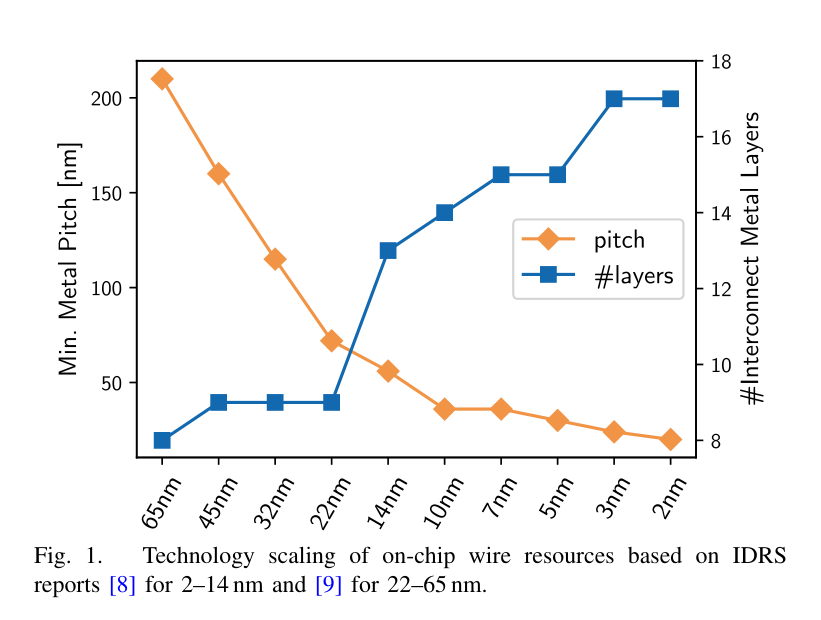
\includegraphics[width=0.65\textwidth]{chapters/ch01-interconnect-crisis/figures/floonoc_fig01_wire_scaling.png}
\caption{Technology scaling of on-chip wire resources based on ITRS/IRDS reports for 2--14~nm and 22--65~nm nodes. While transistor delay decreases exponentially, global wire delay surges. [Reproduced from: T. Fischer, M. Rogenmoser, T. Benz, F. K. G{\"u}rkaynak, and L. Benini, ``FlooNoC: A 645-Gb/s/link 0.15-pJ/B/hop Open-Source NoC With Wide Physical Links and End-to-End AXI4 Parallel Multistream Support,'' \emph{IEEE Trans. Very Large Scale Integr. (VLSI) Syst.}, vol. 33, no. 4, pp. 1094--1107, Apr. 2025~\cite{Fischer2025}. \copyright~2025 IEEE]}
\label{fig:ch1_wire_scaling}
\end{figure}

\subsection{The Mayadas-Shatzkes \& Fuchs-Sondheimer Scattering Models}
\label{subsec:ch1_scattering}

In bulk copper at room temperature, the electron mean free path is $\lambda_0 \approx 39.0$~nm. When the physical width $w$ of an on-chip metal wire shrinks below $2 \lambda_0 \approx 80$~nm, two scattering mechanisms cause the effective resistivity $\rho_{eff}$ to surge dramatically above the bulk value ($\rho_{bulk} \approx 1.68 \times 10^{-8}\ \Omega\cdot\text{m}$):
\begin{enumerate}
    \item \textbf{Surface Scattering (Fuchs-Sondheimer Model)}~\cite{Fuchs1938,Sondheimer1952}: Electrons reflect diffusely off the outer interfaces of the wire:
    \begin{equation}
    \frac{\rho_{FS}}{\rho_{bulk}} = 1 + \frac{3}{8 \kappa} (1 - p)
    \label{eq:fuchs_sondheimer}
    \end{equation}
    where $\kappa = \frac{w_{eff}}{\lambda_0}$ is the normalized wire dimension and $p \in [0, 1]$ is the specularity parameter ($p \approx 0.2$ for realistic barrier interfaces).
    \item \textbf{Grain Boundary Scattering (Mayadas-Shatzkes Model)}~\cite{Mayadas1970}: Nanoscale copper recrystallizes into small grains with average grain diameter $d \approx w_{eff}$. Electrons scatter at grain boundaries:
    \begin{equation}
    \frac{\rho_{MS}}{\rho_{bulk}} = \frac{1}{3 \left[ \frac{1}{3} - \frac{\alpha}{2} + \alpha^2 - \alpha^3 \ln\left(1 + \frac{1}{\alpha}\right) \right]}
    \label{eq:mayadas_shatzkes}
    \end{equation}
    where $\alpha = \frac{\lambda_0}{d} \frac{R}{1 - R}$, with $R \approx 0.3$--$0.5$ representing the grain boundary reflection coefficient.
    \item \textbf{Diffusion Barrier Liner Encroachment}: Copper electromigration requires high-resistivity diffusion liners (Ta/TaN, Co, Ru) of thickness $t_{barrier} \approx 1.0$--$1.5$~nm. Because the liner does not scale down proportionally with the wire trench, the conductive copper cross-sectional area $A_{Cu}$ shrinks much faster than total wire trench area:
    \begin{equation}
    A_{Cu} = (w - 2 t_{barrier}) \cdot (h - t_{barrier}), \qquad \rho_{total} = \rho_{eff} \cdot \left(\frac{w \cdot h}{A_{Cu}}\right)
    \label{eq:barrier_liner}
    \end{equation}
\end{enumerate}

At the 3~nm node ($w \approx 10$~nm), the effective copper resistivity exceeds $15\times$ bulk copper, turning long global wires into unbearable thermal, resistance, and latency bottlenecks.

\subsection{Sub-3nm Transistor Architectures: GAAFET, RibbonFET, and CFET}
\label{subsec:ch1_gaafet}
\index{GAAFET}
\index{RibbonFET}
\index{CFET}

As silicon dimensions scale into the sub-3nm regime, conventional FinFETs encounter severe short-channel degradation and sub-threshold leakage due to quantum confinement limits and corner parasitic leakage. Semiconductor foundries have transitioned to \textbf{Gate-All-Around Field-Effect Transistors (GAAFETs)}~\cite{IntelPowerVia2023} (termed \emph{RibbonFET} by Intel and \emph{MBCFET} by Samsung):
\begin{enumerate}
    \item \textbf{Nanosheet Architecture}: Rather than a vertical 3D silicon fin gated on three sides, a GAAFET comprises multiple horizontally stacked silicon nanosheet ribbons (typically 3 to 4 sheets of thickness $t_{sheet} \approx 5\text{--}6\,\mathrm{nm}$ and width $w_{sheet} \approx 15\text{--}40\,\mathrm{nm}$) completely wrapped by the high-$\kappa$ metal gate dielectric ($HfO_2/TiN$).
    \item \textbf{Sub-Threshold Swing and Electrostatic Control}: Enclosing the channel on all four sides maximizes gate capacitive coupling, driving the sub-threshold swing $S_S$ down to $\approx 64\text{--}67\,\mathrm{mV/decade}$ (near the theoretical thermodynamic limit of $60\,\mathrm{mV/decade}$ at $300\,\mathrm{K}$) and suppressing Drain-Induced Barrier Lowering (DIBL $\le 30\,\mathrm{mV/V}$).
    \item \textbf{Complementary FET (CFET)}: The ultimate scaling evolution of GAAFETs is the \textbf{CFET}, in which an NMOS nanosheet stack is monolithically fabricated \emph{vertically on top} of a PMOS nanosheet stack. By stacking opposite-polarity transistors vertically, standard cell track height shrinks from 5.0T down to 3.0T or 4.0T, doubling transistor density without requiring physical gate pitch reduction.
\end{enumerate}

\subsection{Backside Power Delivery Networks (BSPDN / PowerVia)}
\label{subsec:ch1_bspdn}
\index{Backside Power Delivery (BSPDN)}
\index{PowerVia}

In classical Front-End-of-Line / Back-End-of-Line (FEOL/BEOL) manufacturing, both low-voltage logic signal wires and high-current power distribution rails ($V_{dd}, V_{ss}$) compete for the same frontside metal tracks (M0 through M15). Power routing consumes up to 30\% of intermediate metal tracks, exacerbating routing congestion and inducing severe resistive voltage drop ($IR$-drop).

To overcome this interconnect bottleneck, modern sub-2nm nodes introduce the \textbf{Backside Power Delivery Network (BSPDN)}~\cite{IntelPowerVia2023} (such as Intel PowerVia and TSMC A16):
\begin{itemize}
    \item The wafer is thinned from the backside down to a thickness of $\le 500\,\mathrm{nm}$.
    \item Power delivery networks ($V_{dd}$ and ground grids) are fabricated entirely on the wafer \textbf{backside} using thick, ultra-low-resistance copper layers.
    \item Sub-micron \textbf{Nano-Through-Silicon Vias (nTSVs)} connect backside power rails directly to transistor source/drain terminals.
    \item Frontside metal layers (M0--M14) are freed exclusively for high-density signal interconnects, slashing $IR$-drop by over $30\%$ and increasing signal routing density by up to $20\%$.
\end{itemize}

\subsection{Alternative Interconnect Metallization: Ruthenium, Cobalt, and Molybdenum}
\label{subsec:ch1_alt_metals}
\index{Ruthenium Interconnects}
\index{Cobalt Metallization}
\index{Molybdenum}

Because copper requires high-resistivity diffusion barrier liners (Ta/TaN) that do not scale below $1.0\text{--}1.5\,\mathrm{nm}$, the effective copper conductor area in sub-12nm trenches collapses, triggering catastrophic resistivity surges (Eq.~\ref{eq:barrier_liner}).

To solve this physical scaling wall, semiconductor manufacturers are transitioning the lowest metal levels (M0, M1, M2) from copper to \textbf{linerless refractory and platinum-group metals}~\cite{Adelmann2018}:
\begin{itemize}
    \item \textbf{Ruthenium ($Ru$)}: Ruthenium is a semi-noble metal with high cohesive energy that resists electromigration without requiring any diffusion barrier liner. Crucially, the bulk electron mean free path of ruthenium is only $\lambda_0(Ru) \approx 4.9\,\mathrm{nm}$—nearly \textbf{$8\times$ shorter than copper} ($\lambda_0(Cu) \approx 39.0\,\mathrm{nm}$). Consequently, size-effect grain boundary scattering in ruthenium is drastically attenuated at sub-10nm line widths.
    \item \textbf{Molybdenum ($Mo$) and Cobalt ($Co$)}: Molybdenum exhibits an electron mean free path of $\lambda_0(Mo) \approx 10.0\,\mathrm{nm}$ and low bulk resistivity ($5.3\,\mu\Omega\cdot\mathrm{cm}$), providing superior aspect-ratio fill characteristics without voiding.
\end{itemize}

\begin{figure}[htbp]
\centering
\begin{svgraybox}
\textbf{The Metal Crossover Threshold}: At wire trench widths $w > 15\,\mathrm{nm}$, copper remains superior due to its low bulk resistivity ($1.68\,\mu\Omega\cdot\mathrm{cm}$ vs. $7.1\,\mu\Omega\cdot\mathrm{cm}$ for $Ru$). However, when wire width shrinks below the \textbf{crossover width ($w \le 12\,\mathrm{nm}$)}, the linerless nature and short mean free path of Ruthenium cause its total line resistance to become \textbf{lower than linered copper}, establishing Ruthenium as the future metallization standard for sub-2nm NoC link routers.
\end{svgraybox}
\end{figure}

\subsection{Historical Technology Scaling Across Semiconductor Generations}
\label{subsec:ch1_scaling_table}

Table~\ref{tab:ch1_history} chronicles the physical parameters of interconnect and transistor scaling from the 180nm planar CMOS node to the 2nm GAAFET generation.

\begin{table}[htbp]
\centering
\caption{Comprehensive Interconnect and Transistor Metrics Across Semiconductor Technology Generations}
\label{tab:ch1_history}
\begin{tabular}{lcccccc}
\toprule
\textbf{Node} & \textbf{Year} & \textbf{Device Type} & \textbf{$V_{dd}$ (V)} & \textbf{Min Pitch} & \textbf{Gate Delay} & \textbf{Wire Delay ($1\text{ mm}$)} \\
\midrule
$180\,\mathrm{nm}$ & 1999 & Planar Bulk & 1.80 & $500\,\mathrm{nm}$ & $35.0\,\mathrm{ps}$ & $2.5\,\mathrm{ps}$ \\
$90\,\mathrm{nm}$  & 2003 & Strained Si & 1.20 & $220\,\mathrm{nm}$ & $15.0\,\mathrm{ps}$ & $8.0\,\mathrm{ps}$ \\
$45\,\mathrm{nm}$  & 2007 & High-$\kappa$ Metal & 1.00 & $160\,\mathrm{nm}$ & $7.0\,\mathrm{ps}$  & $25.0\,\mathrm{ps}$ \\
$22\,\mathrm{nm}$  & 2012 & 3D FinFET   & 0.85 & $80\,\mathrm{nm}$  & $3.5\,\mathrm{ps}$  & $90.0\,\mathrm{ps}$ \\
$7\,\mathrm{nm}$   & 2018 & EUV FinFET  & 0.75 & $40\,\mathrm{nm}$  & $1.8\,\mathrm{ps}$  & $350.0\,\mathrm{ps}$ \\
$3\,\mathrm{nm}$   & 2023 & GAAFET      & 0.70 & $24\,\mathrm{nm}$  & $1.1\,\mathrm{ps}$  & $1{,}200.0\,\mathrm{ps}$ \\
$2\,\mathrm{nm}$   & 2025 & RibbonFET/BSPDN & 0.65 & $18\,\mathrm{nm}$ & $0.8\,\mathrm{ps}$  & $2{,}800.0\,\mathrm{ps}$ \\
\bottomrule
\end{tabular}
\end{table}

As documented in Table~\ref{tab:ch1_history}, while gate delay dropped by over \textbf{$43\times$} from 180nm to 2nm, unrepeated wire delay across a 1\,mm global span escalated by more than \textbf{$1{,}100\times$}. This catastrophic divergence provides the definitive physical justification for packet-switched Networks-on-Chip.

\section{High-Frequency Transmission Line Effects and Inductive Peaking}
\label{sec:ch1_transmission_lines}

As clock frequencies exceed $2\text{--}4\,\mathrm{GHz}$ and signal rise times $t_r$ compress below $30\text{--}50\,\mathrm{ps}$, on-chip global wires cease to behave as purely diffusive distributed $RC$ circuits and transition into distributed $RLC$ transmission lines~\cite{DallyPoulton1998}. When the signal transition time $t_r$ is comparable to the electromagnetic time of flight $t_f = L \sqrt{\mathcal{L} \cdot \mathcal{C}}$, inductive reactance $\omega \mathcal{L}$ rivals series resistance $\mathcal{R}$, inducing reflection ringing, inductive crosstalk, and signal overshoot.

\subsection{The Telegrapher's Equations and the Wave Equation}
\label{subsec:ch1_telegraphers}

A transmission line is governed by the classical Telegrapher's equations:
\begin{align}
-\frac{\partial v(x, t)}{\partial x} &= \mathcal{R} \cdot i(x, t) + \mathcal{L} \cdot \frac{\partial i(x, t)}{\partial t} \label{eq:ch1_telegrapher_v} \\
-\frac{\partial i(x, t)}{\partial x} &= \mathcal{G} \cdot v(x, t) + \mathcal{C} \cdot \frac{\partial v(x, t)}{\partial t} \label{eq:ch1_telegrapher_i}
\end{align}
where $\mathcal{R}$ ($\Omega/\mathrm{m}$), $\mathcal{L}$ ($\mathrm{H/m}$), $\mathcal{G}$ ($\mathrm{S/m}$), and $\mathcal{C}$ ($\mathrm{F/m}$) denote per-unit-length series resistance, loop inductance, dielectric conductance, and shunt capacitance, respectively. Differentiating with respect to spatial coordinate $x$ yields the lossy wave equation:
\begin{equation}
\frac{\partial^2 v(x, t)}{\partial x^2} = \mathcal{L}\mathcal{C} \frac{\partial^2 v(x, t)}{\partial t^2} + (\mathcal{R}\mathcal{C} + \mathcal{L}\mathcal{G}) \frac{\partial v(x, t)}{\partial t} + \mathcal{R}\mathcal{G} v(x, t)
\label{eq:ch1_wave_equation}
\end{equation}

The transition criterion from the diffusive $RC$ regime to the wave-propagation $RLC$ regime is established by comparing the wire length $L$ to the attenuation attenuation length and signal rise time:
\begin{equation}
\text{RLC Effects Significant} \iff t_r \le 2.5 \cdot t_f = 2.5 \cdot L \sqrt{\mathcal{L}\mathcal{C}} \quad \text{and} \quad \mathcal{R} \cdot L \le 2 Z_0
\label{eq:ch1_rlc_condition}
\end{equation}
where $Z_0 = \sqrt{\mathcal{L}/\mathcal{C}}$ is the characteristic impedance of the lossless transmission line. In intermediate metal layers ($M_4\text{--}M_7$), high series resistance ($\mathcal{R} \gg \omega \mathcal{L}$) damps inductive waves, keeping lines in the $RC$ regime. However, in top-level global redistribution layers (thick metal $M_{top}$, $h \ge 1.5\,\mu\mathrm{m}$, $w \ge 1.0\,\mu\mathrm{m}$), series resistance drops to $\mathcal{R} \le 20\,\Omega/\mathrm{mm}$ while loop inductance reaches $\mathcal{L} \approx 0.5\text{--}1.0\,\mathrm{nH/mm}$. Under these conditions, wire propagation speed approaches the speed of light in silicon dioxide ($v = c / \sqrt{\epsilon_r} \approx 150\,\mu\mathrm{m/ps}$), but un-terminated lines suffer severe reflections with reflection coefficient $\Gamma_L = \frac{R_L - Z_0}{R_L + Z_0}$.

\subsection{High-Frequency Skin Effect and Dielectric Loss}
\label{subsec:ch1_skin_effect}

At multi-gigahertz frequencies, alternating magnetic fields force current toward the outer conductor perimeter, confining conduction to a characteristic skin depth $\delta$:
\begin{equation}
\delta = \sqrt{\frac{\rho}{\pi \cdot f \cdot \mu_0 \cdot \mu_r}}
\label{eq:ch1_skin_depth}
\end{equation}
For copper ($\rho = 1.68 \times 10^{-8}\,\Omega\cdot\mathrm{m}$, $\mu_r = 1$), the skin depth is $\delta \approx 0.95\,\mu\mathrm{m}$ at $5\,\mathrm{GHz}$ and shrinks to $\delta \approx 0.67\,\mu\mathrm{m}$ at $10\,\mathrm{GHz}$. When conductor thickness exceeds $2\delta$, current crowding raises the effective AC resistance:
\begin{equation}
\mathcal{R}_{AC}(f) \approx \mathcal{R}_{DC} \cdot \left[ 1 + \left(\frac{f}{f_{skin}}\right)^2 \right]^{1/4} \propto \sqrt{f}
\label{eq:ch1_ac_resistance}
\end{equation}
Concurrently, dielectric polarization lag in the low-$k$ inter-layer dielectric introduces a loss tangent $\tan \delta_{diel}$:
\begin{equation}
\mathcal{G}(f) = 2 \pi f \cdot \mathcal{C} \cdot \tan \delta_{diel}
\label{eq:ch1_dielectric_loss}
\end{equation}
Together, skin-effect attenuation and dielectric absorption severely attenuate the high-frequency harmonics of digital clock and data edges, causing eye-diagram closure on long unbuffered buses.

\section{The Monolithic Crossbar and Its Quadratic Area Explosion}
\label{sec:ch1_crossbar}

To avoid the serialized contention of a single shared bus, architects initially considered a full centralized crossbar switch connecting $N$ masters directly to $M$ slaves~\cite{Passas2012}. While a crossbar allows non-interfering parallel communication between disjoint pairs of masters and slaves, its hardware complexity scales quadratically:
\begin{equation}
\text{Crosspoints} = N \times M \approx O(N^2), \qquad \text{Wiring Tracks} = (N + M) \times W_{data\_width} \approx O(N)
\label{eq:crossbar_complexity}
\end{equation}
For an MPSoC with $N = 64$ cores, a full crossbar requires $64 \times 64 = 4,096$ crosspoint multiplexer switches and $128 \times 128 = 16,384$ wires crossing a central silicon layout area, causing severe layout congestion, routing track starvation, and parasitic capacitive coupling crosstalk. A full crossbar switch is physically viable only for small clusters ($N \le 4$--$8$ cores).

\section{Optimal Repeater Insertion Theory (Bakoglu's Formulation)}
\label{sec:ch1_repeaters}

To counteract the quadratic delay growth of long $RC$ lines ($\tau \propto L^2$), designers segment wires by inserting CMOS inverters or non-inverting buffers (repeaters) at regular intervals~\cite{Bakoglu1990}. By partitioning a line of length $L$ into $k$ equal segments of length $l = L/k$, each driven by a buffer sized $h$ times the minimum-sized inverter, the delay transforms from quadratic to linear in total length:
\begin{equation}
\tau_{total} = k \cdot \tau_{segment} = \frac{L}{l} \cdot \left[ R_0 \cdot \left( \frac{\mathcal{C} \cdot l}{h} + C_0 \right) + \frac{\mathcal{R} \cdot l}{h} \cdot C_0 + \frac{1}{2} \mathcal{R}\mathcal{C} \cdot l^2 \right]
\label{eq:ch1_repeater_delay}
\end{equation}
where $R_0$ and $C_0$ are the output drive resistance and input gate capacitance of a minimum-sized inverter ($h=1$), and $\mathcal{R}, \mathcal{C}$ are the per-unit-length wire resistance and capacitance.

By setting the partial derivatives $\frac{\partial \tau_{total}}{\partial l} = 0$ and $\frac{\partial \tau_{total}}{\partial h} = 0$, Bakoglu~\cite{Bakoglu1990} derived the closed-form optimal repeater spacing $l_{opt}$ and buffer sizing factor $h_{opt}$:
\begin{align}
l_{opt} &= \sqrt{\frac{2 R_0 C_0}{\mathcal{R} \cdot \mathcal{C}}} \label{eq:ch1_l_opt} \\
h_{opt} &= \sqrt{\frac{R_0 \cdot \mathcal{C}}{\mathcal{R} \cdot C_0}} \label{eq:ch1_h_opt}
\end{align}

Substituting Eq.~(\ref{eq:ch1_l_opt}) and Eq.~(\ref{eq:ch1_h_opt}) into Eq.~(\ref{eq:ch1_repeater_delay}) yields the minimum achievable interconnect propagation delay per unit length:
\begin{equation}
\left( \frac{\tau}{L} \right)_{min} = 2 \sqrt{R_0 C_0 \cdot \mathcal{R}\mathcal{C}} \cdot \left( 1 + \sqrt{\frac{1}{2}} \right) \approx 2.41 \cdot \sqrt{R_0 C_0 \cdot \mathcal{R}\mathcal{C}}
\label{eq:ch1_min_delay_per_mm}
\end{equation}

\begin{svgraybox}
\textbf{The Repeater Insertion Dilemma}: While optimal repeater insertion linearizes wire delay, it imposes severe silicon area and power penalties:
\begin{itemize}
    \item \textbf{Active Silicon Tax}: For a 1024-bit bus traversing a $20\,\mathrm{mm}$ die, optimal repeaters consume over $12\%$ of active silicon area in intermediate tiers.
    \item \textbf{Dynamic Switching Power}: $P_{dyn} = k \cdot (h \cdot C_0 + \mathcal{C} \cdot l_{opt}) \cdot V_{dd}^2 \cdot f$, dissipating gigawatts of unrecoverable charging energy across global links.
    \item \textbf{Bidirectional Routing Obstacles}: Repeaters are unidirectional CMOS amplifiers; bidirectional buses require complex tri-state transceivers and direction-control routing.
\end{itemize}
\end{svgraybox}

\section{The Network-on-Chip Paradigm: Packet-Switched Modular Interconnects}
\label{sec:ch1_noc_paradigm}

In 2001, pioneering papers by Dally \& Towles (\emph{``Route Packets, Not Wires''}~\cite{Dally2001}) and Benini \& De Micheli (\emph{``Networks on Chips: A New SoC Paradigm''}~\cite{Benini2002}) introduced the definitive architectural solution:
\begin{svgraybox}
\textbf{The Network-on-Chip (NoC) Principle}: Replace long, dedicated, unstructured global metal wires with a structured, packet-switched micro-network composed of modular routers and short, pipelined point-to-point links.
\end{svgraybox}

Key advantages of the NoC architecture include:
\begin{enumerate}
    \item \textbf{Bounded Wire Lengths}: Every link connects strictly adjacent routers. The link wire length is fixed to the physical pitch of one compute tile ($L_{link} \approx 0.5$--$1.5$~mm), regardless of whether the chip contains 16 or 2,048 cores.
    \item \textbf{Predictable Timing \& Pipelining}: Because link wire delay is short and localized, routers and links can be clocked at high frequencies ($f_{clk} \approx 1.5$--$2.5$~GHz) without repeater insertion crises.
    \item \textbf{Concurrent Multi-Hop Communication}: Multiple packets traverse non-overlapping segments of the network simultaneously, yielding aggregate throughput that scales proportionally with the network size:
    \begin{equation}
    BW_{bisection} \propto \sqrt{N} \times W_{link} \times f_{clk}
    \label{eq:bisection_bw}
    \end{equation}
    \item \textbf{Modularity \& Silicon Reuse}: Adding processing tiles does not require redesigning the global wiring tree.
\end{enumerate}

\section{Industrial Case Studies: From 48 Cores to Wafer-Scale Engines}
\label{sec:ch1_case_studies}

To examine the real-world execution of NoC architecture in modern silicon, we analyze landmark implementations across academic and industrial milestones:

\subsection{The Intel TeraFLOPS 80-Core Processor (65nm CMOS)}
\label{subsec:ch1_intel_80core}

Fabricated by Intel in 2007 (Vangal et al., ISSCC)~\cite{Vangal2008}, the TeraFLOPS processor represented the world's first microprocessor to achieve $1.0\,\mathrm{TFLOPS}$ double-precision floating-point performance on a single chip. It featured an $8 \times 10$ 2D mesh of compute tiles running at $4.0\,\mathrm{GHz}$ at $1.2\,\mathrm{V}$ ($62\,\mathrm{W}$). Each tile contained a 5-port 5-stage pipelined packet-switched router with crossbar switch bandwidth of $80\,\mathrm{GB/s}$ per node, providing an unprecedented $1.6\,\mathrm{Tb/s}$ of bisection bandwidth across short, regular $1.2\,\mathrm{mm}$ point-to-point links.

\subsection{The Tilera TILE64 Manycore Processor (90nm CMOS)}
\label{subsec:ch1_tilera64}

The Tilera TILE64 architecture departed from traditional single-mesh NoCs by implementing \textbf{five independent, concurrent physical 2D mesh networks} on the same silicon die~\cite{Wentzlaff2007}:
\begin{enumerate}
    \item \textbf{UDI (User Dynamic Interconnect)}: Zero-overhead streaming user-level message passing between processor cores.
    \item \textbf{IDN (I/O Dynamic Interconnect)}: Dedicated DMA transfers from PCIe and 10GbE network interfaces to on-chip tile SRAM caches.
    \item \textbf{MDN (Memory Dynamic Interconnect)}: Cache-to-DDR memory controller request and response channels.
    \item \textbf{TDN (Tile Dynamic Interconnect)}: Coherent L2 cache-to-cache intervention and invalidation traffic.
    \item \textbf{STN (Static Interconnect)}: Circuit-switched deterministic real-time communication.
\end{enumerate}
By separating traffic into independent physical networks, the TILE64 completely prevented cache coherence transactions from being delayed by bulk I/O streaming, delivering over $30\,\mathrm{Tb/s}$ of aggregate bisection throughput.

\subsection{The Cerebras Wafer-Scale Engine (WSE-2 \& WSE-3)}
\label{subsec:ch1_cerebras}

The Cerebras Wafer-Scale Engine represents the extreme physical limit of monolithic Network-on-Chip scaling~\cite{Lie2022}. Rather than cutting wafers into individual dies, Cerebras fabricates an entire $300\,\mathrm{mm}$ silicon wafer as a single contiguous compute system:
\begin{itemize}
    \item \textbf{Core Count}: $850,000$ AI-optimized tensor processing cores (WSE-2) and $900,000$ cores in 5nm (WSE-3).
    \item \textbf{Wafer-Scale Interconnect}: The chip-cutting boundary (scribe lines) is bridged using dedicated high-density lithographic cross-reticle metal lines, creating a seamless 2D mesh fabric spanning $46,225\,\mathrm{mm^2}$.
    \item \textbf{On-Chip Fabric Bandwidth}: The contiguous 2D mesh fabric delivers over $\mathbf{220\,\mathrm{Pb/s}}$ (petabits per second) of internal fabric bandwidth with single-cycle router latency per hop.
    \item \textbf{Hardware Redundancy}: A built-in fault-tolerant bypass fabric automatically detects and routes around defective fabrication sites, ensuring $100\%$ operational yield on a wafer with thousands of native silicon defect points.
\end{itemize}

To examine the real-world execution of NoC architecture in modern silicon, we analyze landmark implementations from our literature corpus:

\subsection{The 2,048-Core HammerBlade Manycore SoC (12nm FinFET)}
\label{subsec:ch1_hammerblade}

A landmark demonstration of extreme monolithic scaling is the \textbf{HammerBlade (HB)} processor developed by Gao et al.~\cite{Gao2026} and Davidson et al.~\cite{Davidson2023}.

\begin{figure}[t]
\centering
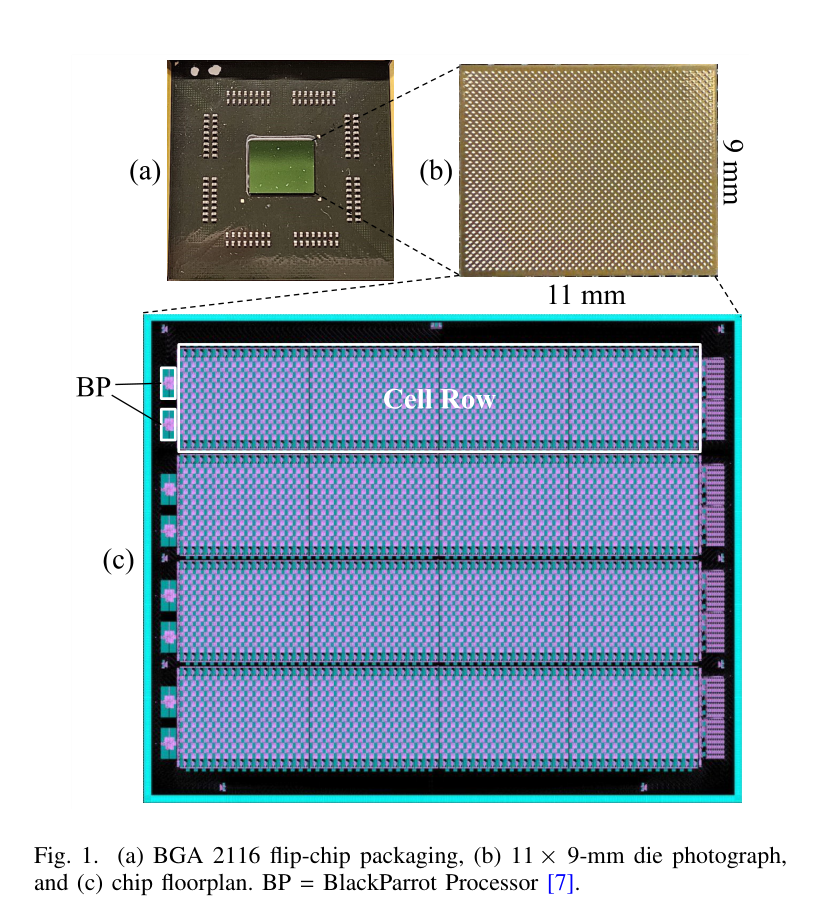
\includegraphics[width=0.92\textwidth]{chapters/ch01-interconnect-crisis/figures/hammerblade_fig01_die_floorplan.png}
\caption{Modern monolithic manycore scaling in 12nm silicon: (a) BGA 2116 flip-chip packaging, (b) $11 \times 9$-mm die photograph, and (c) chip floorplan of the 2,048-core HammerBlade SoC. [Reproduced from: P. Gao et al., ``HammerBlade in Silicon: A 12-nm 2048-Core RISC-V Manycore SoC With Ruche Networks,'' \emph{IEEE Trans. Very Large Scale Integr. (VLSI) Syst.}, vol. 34, no. 7, pp. 2306--2310, July 2026~\cite{Gao2026}. \copyright~2026 IEEE]}
\label{fig:ch1_hammerblade_die}
\end{figure}

\begin{figure}[t]
\sidecaption[t]
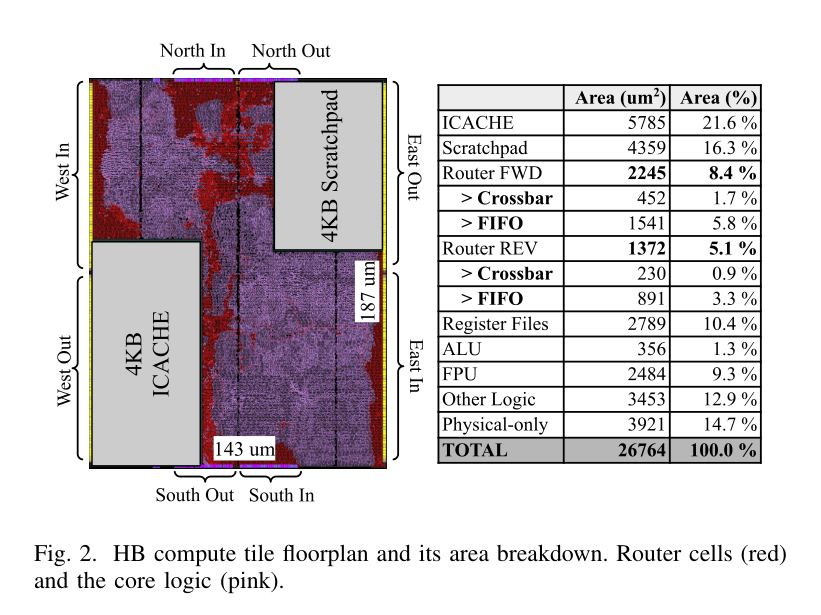
\includegraphics[width=0.65\textwidth]{chapters/ch01-interconnect-crisis/figures/hammerblade_fig02_tile_floorplan.png}
\caption{HammerBlade compute tile floorplan and physical area breakdown showing router cells (red) and core logic (pink). [Reproduced from: P. Gao et al., ``HammerBlade in Silicon: A 12-nm 2048-Core RISC-V Manycore SoC With Ruche Networks,'' \emph{IEEE Trans. Very Large Scale Integr. (VLSI) Syst.}, vol. 34, no. 7, pp. 2306--2310, July 2026~\cite{Gao2026}. \copyright~2026 IEEE]}
\label{fig:ch1_hammerblade_tile}
\end{figure}

Key architectural and physical metrics of the HammerBlade processor include:
\begin{itemize}
    \item \textbf{Silicon Area}: $99\text{ mm}^2$ in TSMC 12nm FinFET.
    \item \textbf{Compute Density}: 2,048 custom RISC-V cores organized into an array of $64 \times 32$ tiles.
    \item \textbf{Interconnect Topology}: \textbf{Ruche Network}, a wire-maximal topology overlaying nearest-neighbor 2D mesh links with long-distance multi-hop bypass express wires.
    \item \textbf{Clocking \& Throughput}: Operating at \textbf{1.49~GHz at 0.8~V}, the NoC delivers a peak aggregate bandwidth of \textbf{2,572.6 Tb/s} and a bisection bandwidth of \textbf{53.2 Tb/s}.
    \item \textbf{Routing Density}: Achieves \textbf{4,289 bit/mm} across higher metal layers.
    \item \textbf{Integration}: Leverages \textbf{On-Chip Source-Synchronous Interconnect (OCSSI)} under a Globally Asynchronous Locally Synchronous (GALS) paradigm to eliminate chip-wide clock tree skew.
\end{itemize}

\begin{table}[t]
\caption{Evolution of Silicon Landmark Network-on-Chip Processors}
\label{tab:noc_evolution}
\begin{tabular}{p{2.8cm}p{1.8cm}p{1.8cm}p{2.0cm}p{2.0cm}p{2.2cm}}
\hline\noalign{\smallskip}
Architecture & Year / Venue & Process Node & Tile Array / Cores & Peak Bisection BW & Interconnect Topology \\
\noalign{\smallskip}\svhline\noalign{\smallskip}
Intel TeraFLOPS & 2008 JSSC~\cite{Vangal2008} & 65nm Bulk & $8\times 10$ (80) & 1.6 Tb/s & 2D Mesh (5-port) \\
Intel 48-Core SCC & 2011 JSSC~\cite{Howard2011} & 45nm Bulk & $6\times 4$ (48) & 256 Gb/s & 2D Mesh (e-cube) \\
Kalray MPPA-256 & 2013 HPEC~\cite{Dinechin2013} & 28nm CMOS & 16 Clusters & 384 Gb/s & 2D Torus \\
Theseus WSC & 2025 TCAD~\cite{Zhu2025} & Wafer-Scale & Wafer Grid & 100+ Tb/s & 2D Torus Wafer NoC \\
FlooNoC (Benini) & 2025 TVLSI~\cite{Fischer2025} & 12nm FinFET & $8\times 4$ (288) & 103 Tb/s & Wide AXI4 2D Mesh \\
HammerBlade (Gao)& 2026 TVLSI~\cite{Gao2026} & 12nm FinFET & $64\times 32$ (2,048) & 53.2 Tb/s & Ruche Multi-Hop NoC \\
\noalign{\smallskip}\hline\noalign{\smallskip}
\end{tabular}
\end{table}

\subsection{Physics-Based Electromigration Reliability in Sub-10nm Interconnects}
\label{sec:ch1_electromigration}
As wire geometries scale deep into sub-10~nm regimes, interconnect degradation driven by high current densities and thermo-mechanical stress becomes a primary limiting factor for chip longevity. Electromigration (EM) induces atomic momentum transfer from conducting electrons to metal lattice atoms, leading to void formation at cathode ends and hillocks/short-circuits at anode terminals. Traditional EM analysis relies on conservative empirical models (Black's equation) that lack spatial and dynamic granularity across full-chip network traces. Recent physics-based analytical techniques formulated by Wang et al.~\cite{Wang2021EM} introduce efficient eigenfunction-based transient solutions for hydrostatic stress evolution in multi-branch interconnect trees. By decoupling boundary value problems into closed-form eigen-mode expansions, transient atomic drift and stress buildup can be evaluated orders of magnitude faster than conventional finite-element methods (FEM), enabling real-time reliability-aware routing and power-grid co-design in modern NoC fabrics.

\section{Interactive Lab \& Hands-on Challenges}
\label{sec:ch1_interactive}

To build an experimental understanding of interconnect trade-offs, explore the companion simulators on the \textbf{NoC Learning Hub} (\url{https://network-on-chip.github.io/learning/}):
\begin{itemize}
    \item \textbf{2D Mesh Routing Visualizer} (\url{https://network-on-chip.github.io/learning/interactive/visualizer/}): Inject uniform random and hotspot traffic into a $4 \times 4$ and $8 \times 8$ mesh; observe how localized point-to-point links sustain continuous throughput without centralized bus stalls.
    \item \textbf{Topology Titans: Graph Architect} (\url{https://network-on-chip.github.io/learning/interactive/topology/}): Synthesize 2D Mesh, 2D Torus, and Hypercube topologies within strict wire length and pin degree limits.
    \item \textbf{Arbiter Arena: Crossbar Clash} (\url{https://network-on-chip.github.io/learning/interactive/arbiter/}): Benchmark matrix, round-robin, and wavefront arbiters under heavy contention.
\end{itemize}

\section{Checkpoint Assessment}
\label{sec:ch1_assessment}

\begin{enumerate}
    \item \textbf{Question 1.1 (Tier 1: Fundamental)}: Why does the propagation delay of a shared multi-drop bus grow as $O(N^{3/2})$ to $O(N^2)$ as core count $N$ scales, rather than remaining constant?
    \item \textbf{Question 1.2 (Tier 2: Architectural Analysis)}: What is the Mayadas-Shatzkes effect, and why does it represent a critical barrier for on-chip global interconnects below 14~nm?
    \item \textbf{Question 1.3 (Tier 3: Design Trade-Off)}: Why is a centralized $N \times N$ crossbar switch unacceptable for a 128-core processor, despite offering non-blocking zero-hop communication between disjoint pairs?
\end{enumerate}
\emph{Detailed answers and derivations for these questions are provided in the Solutions chapter at the end of this volume.}

\section{References \& Further Reading}
\label{sec:ch1_references}

\begin{enumerate}
    \item \textbf{[Moore1965]} G.~E.~Moore, ``Cramming More Components Onto Integrated Circuits,'' \emph{Electronics}, vol.~38, no.~8, pp.~114--117, 1965. \url{https://doi.org/10.1109/JPROC.1998.658762}
    \item \textbf{[Dennard1974]} R.~H.~Dennard, F.~H.~Gaensslen, H.-N.~Yu, V.~L.~Rideout, E.~Bassous, and A.~R.~LeBlanc, ``Design of Ion-Implanted MOSFET's with Very Small Physical Dimensions,'' \emph{IEEE Journal of Solid-State Circuits}, vol.~SC-9, no.~5, pp.~256--268, 1974. \url{https://doi.org/10.1109/JSSC.1974.1052523}
    \item \textbf{[Borkar1999]} S.~Borkar, ``Design Challenges of Technology Scaling,'' \emph{IEEE Micro}, vol.~19, no.~4, pp.~23--29, 1999. \url{https://doi.org/10.1109/40.782564}
    \item \textbf{[Ho2001]} R.~Ho, K.~W.~Mai, and M.~A.~Horowitz, ``The Future of Wires,'' \emph{Proceedings of the IEEE}, vol.~89, no.~4, pp.~490--504, 2001. \url{https://doi.org/10.1109/5.920580}
    \item \textbf{[Mayadas1970]} A.~F.~Mayadas and M.~Shatzkes, ``Electrical-Resistivity Model for Polycrystalline Films: The Case of Arbitrary Reflection at External Surfaces,'' \emph{Physical Review B}, vol.~1, no.~4, pp.~1382--1389, 1970. \url{https://doi.org/10.1103/PhysRevB.1.1382}
    \item \textbf{[Fuchs1938]} K.~Fuchs, ``The Conductivity of Thin Metallic Films According to the Electron Theory of Metals,'' \emph{Mathematical Proceedings of the Cambridge Philosophical Society}, vol.~34, no.~1, pp.~100--108, 1938. \url{https://doi.org/10.1017/S0305004100019952}
    \item \textbf{[Sondheimer1952]} E.~H.~Sondheimer, ``The Mean Free Path of Electrons in Metals,'' \emph{Advances in Physics}, vol.~1, no.~1, pp.~1--42, 1952. \url{https://doi.org/10.1080/00018735200101151}
    \item \textbf{[Elmore1948]} W.~C.~Elmore, ``The Transient Response of Damped Linear Networks with Particular Regard to Wideband Amplifiers,'' \emph{Journal of Applied Physics}, vol.~19, no.~1, pp.~55--63, 1948. \url{https://doi.org/10.1063/1.1697872}
    \item \textbf{[Bakoglu1990]} H.~B.~Bakoglu, \emph{Circuits, Interconnections, and Packaging for VLSI}, Reading, MA: Addison-Wesley, 1990.
    \item \textbf{[DallyPoulton1998]} W.~J.~Dally and J.~W.~Poulton, \emph{Digital Systems Engineering}, Cambridge: Cambridge University Press, 1998. \url{https://doi.org/10.1017/CBO9780511805172}
    \item \textbf{[Passas2012]} G.~Passas, M.~Katevenis, and D.~Pnevmatikatos, ``Crossbar NoCs Are Scalable Beyond 100 Nodes,'' \emph{IEEE Transactions on Computer-Aided Design of Integrated Circuits and Systems}, vol.~31, no.~4, pp.~573--585, 2012. \url{https://doi.org/10.1109/TCAD.2011.2176730}
    \item \textbf{[Dally2001]} W.~J.~Dally and B.~Towles, ``Route Packets, Not Wires: On-Chip Interconnection Networks,'' in \emph{Proceedings of the 38th Annual Design Automation Conference (DAC)}, 2001, pp.~684--689. \url{https://doi.org/10.1145/378239.379048}
    \item \textbf{[Benini2002]} L.~Benini and G.~De Micheli, ``Networks on Chips: A New SoC Paradigm,'' \emph{IEEE Computer}, vol.~35, no.~1, pp.~70--78, 2002. \url{https://doi.org/10.1109/2.976921}
    \item \textbf{[Vangal2008]} S.~R.~Vangal et al., ``An 80-Tile Sub-100-W TeraFLOPS Processor in 65-nm CMOS,'' \emph{IEEE Journal of Solid-State Circuits}, vol.~43, no.~1, pp.~29--41, 2008. \url{https://doi.org/10.1109/JSSC.2007.910957}
    \item \textbf{[Wentzlaff2007]} D.~Wentzlaff et al., ``On-Chip Interconnection Architecture of the Tile Processor,'' \emph{IEEE Micro}, vol.~27, no.~5, pp.~15--31, 2007. \url{https://doi.org/10.1109/MM.2007.89}
    \item \textbf{[Howard2011]} J.~Howard et al., ``A 48-Core IA-32 Message-Passing Processor with DVFS in 45nm CMOS,'' \emph{IEEE Journal of Solid-State Circuits}, vol.~46, no.~1, pp.~173--183, 2011. \url{https://doi.org/10.1109/JSSC.2010.2079496}
    \item \textbf{[Dinechin2013]} B.~D.~de Dinechin et al., ``A Distributed Run-Time Environment for the Kalray MPPA-256 Manycore Processor,'' in \emph{Proceedings of the IEEE High Performance Extreme Computing Conference (HPEC)}, 2013, pp.~1--6. \url{https://doi.org/10.1109/HPEC.2013.6670342}
    \item \textbf{[Lie2022]} S.~Lie, ``Cerebras Architecture Deep Dive: First-Principles Wafer-Scale AI Acceleration,'' \emph{IEEE Micro}, vol.~43, no.~3, pp.~18--30, 2023. \url{https://doi.org/10.1109/MM.2023.3259837}
    \item \textbf{[Fischer2025]} T.~Fischer, M.~Rogenmoser, T.~Benz, F.~K.~G{\"{u}}rkaynak, and L.~Benini, ``FlooNoC: A 645-Gb/s/link 0.15-pJ/B/hop Open-Source NoC With Wide Physical Links and End-to-End AXI4 Parallel Multistream Support,'' \emph{IEEE Transactions on Very Large Scale Integration (VLSI) Systems}, vol.~33, no.~4, pp.~1094--1107, 2025. \url{https://doi.org/10.1109/TVLSI.2025.3527225}
    \item \textbf{[Gao2026]} P.~Gao et al., ``HammerBlade in Silicon: A 12-nm 2048-Core RISC-V Manycore SoC With Ruche Networks,'' \emph{IEEE Transactions on Very Large Scale Integration (VLSI) Systems}, vol.~34, no.~7, pp.~2306--2310, 2026. \url{https://doi.org/10.1109/TVLSI.2026.3684311}
    \item \textbf{[Zhu2025]} J.~Zhu et al., ``Theseus: Exploring Efficient Wafer-Scale Chip Design for Large Language Models,'' \emph{IEEE Transactions on Computer-Aided Design of Integrated Circuits and Systems}, vol.~44, no.~11, pp.~3810--3823, 2025. \url{https://doi.org/10.1109/TCAD.2024.3496321}
    \item \textbf{[AlAlousi2026]} A.~Al-Alousi, M.~Li, and H.~Meng, ``Vendor-Independent Design Space Exploration and Resource Optimization Framework for 3-D Networks-on-Chip Using Hypergraph-Genetic Algorithm Integration,'' \emph{IEEE Transactions on Computer-Aided Design of Integrated Circuits and Systems}, vol.~45, no.~5, pp.~2236--2248, 2026. \url{https://doi.org/10.1109/TCAD.2025.3616073}
    \item \textbf{[Wang2021EM]} Z.~Wang, S.~Zhang, and S.~X.-D.~Tan, ``Fast Physics-Based Electromigration Analysis for Full-Chip Networks by Efficient Eigenfunction-Based Solution,'' \emph{IEEE Transactions on Computer-Aided Design of Integrated Circuits and Systems}, vol.~40, no.~9, pp.~1885--1898, 2021. \url{https://doi.org/10.1109/TCAD.2020.3020641}

    \item \textbf{[Adelmann2018]} C.~Adelmann, K.~Sankaran, S.~Dutta, C.~J.~Wilson, G.~Pourtois, and J.~B{\"o}mmels, ``Alternative Metals for Advanced Interconnects, in \emph{Proceedings of the IEEE International Interconnect Technology Conference (IITC)}, 2018, pp.~133--135. \url{https://doi.org/10.1109/IITC-AMG.2018.8687796}
    \item \textbf{[Davidson2023]} S.~Davidson et al., ``The Bespoke Silicon Group HammerBlade Manycore Architecture, \emph{IEEE Micro}, vol.~43, no.~3, pp.~45--56, May-June 2023. \url{https://doi.org/10.1109/MM.2023.3248834}
    \item \textbf{[IntelPowerVia2023]} E.~S. et al., ``Intel PowerVia Technology: Backside Power Delivery for High Performance Computing, in \emph{Symposium on VLSI Technology and Circuits}, 2023, pp.~1--2. \url{https://doi.org/10.23919/VLSITechnologyandCir57934.2023.10185289}
\end{enumerate}
